\documentclass[a4paper,openright,12pt]{report}

%
% Times New Roman font.
%
\usefont{T1}{ptm}{m}{n}
\selectfont


% Packages a utilizar e respetivos parâmetros.
\usepackage{indentfirst}
\usepackage{inputenc}
\usepackage{enumitem}
\usepackage[english]{babel}
\usepackage{graphicx}
\usepackage{float}
\usepackage{url}

\makeatletter
\let\NAT@parse\undefined
\makeatother
\usepackage{hyperref}

\addto{\captionsenglish}{\renewcommand{\bibname}{References}}
% Definições das dimensões das páginas
\setlength{\textheight}{24.00cm}
\setlength{\textwidth}{15.50cm}
\setlength{\topmargin}{0.35cm}
\setlength{\headheight}{0cm}
\setlength{\headsep}{0cm}
\setlength{\oddsidemargin}{0.25cm}
\setlength{\evensidemargin}{0.25cm}

%
% Times New Roman font.
%
\usefont{T1}{ptm}{m}{n}
\selectfont

%
%title
%
\title{%
  \vspace{-55mm}
  \begin{minipage}[l]{150mm}
    \resizebox{50mm}{!}{
\includegraphics{./figures/logo_isel.png}}
  \end{minipage}\\
  \vspace{20mm}
  \textbf{Corporate Collaboration}
}

%
%authors
%
\author{%
  \begin{tabular}{ll}
      & David Fidalgo \\
      & goncalo9marco@hotmail.com\\
      & 968 225 962
  \\\\
    & Pedro Santos \\
    & santos.pedroc@gmail.com \\
    & 962 942 930
  \\\\
    & Valdemar Antunes \\
    & ValdemarPCA@hotmail.com \\
    & 966 439 259
  \end{tabular}
} 

%
% date
%
\date{%
\vspace{30mm}
\begin{center}
  \begin{tabular}{cc}
    & {Orientadores:} \\
    & Paula Graça, ISEL, paula.graca@isel.pt \\
    & Diogo Pacheco, Do iT Lean, diogo.pacheco@doitlean.com\\
  \end{tabular}\\
\end{center}
\vspace{20mm}
Proposta de projeto realizado no âmbito de Projecto e Seminário,\\
do curso de licenciatura em Engenharia Informática e de Computadores\\
Semestre de Verão 2019/2020
\vspace{10mm}\\
14 de Março de 2020}

\begin{document}
\thispagestyle{empty}
\maketitle
\section*{Introduction}
 Today's market, increasingly technological, demanding and challenging, imposes a work rhythm on companies,
 that besides managing their core business processes, also have a significant amount of dynamics on internal
 activities to help them in their growth and competitiveness. 
 In particular, companies in the information and technologies sector keep internal activities such as work fairs, 
 knowledge sharing through informal presentations, software components development, qualification opportunities, 
 playful activities, among others. In order to put these activities in practice, in an efficient way, 
 there must be a coordination of resources that is not easy to obtain, given its allocation to ongoing projects. 
 \par However, by developing a collaboration platform we can achieve correct management of the plannings, 
 so that they can be executed in due time, and the whole process can be agile allowing, 
 not only the registration and publication of internal needs, 
 but also the acceptance of applications by the collaborators interested in its development. 
 Therefore, it is intended to develop a web reactive application using the OutSystems platform [1], 
 that functions as a collaboration platform designed for the management of internal corporate necessities in a company, 
 and is accessible in all kinds of devices: browsers, tablets and smartphones.
    
    
\section*{Requirements}

In order to create a fully functional, efficient and trustworthy reactive web application that will 
work as a collaboration platform for companies to use, 
there must be a set of requirements that are predefined in due time. 
The understanding of the OutSystems platform and the exploration of its usability is a key factor 
that will provide a concise implementation of these requirements. 
The main requirements are as follows:
  
\begin{enumerate}
\item Registration and authentication in the collaboration platform.
\item Registration of the company's internal necessities, such as the planning of events or job fairs, brown bags to share knowledge between employees, right medium posts, qualification offers, software components development, internal opportunities for career progression and off work activities.
\item Disclosure and scheduling of the company's necessities.
\item Application management and registration for the divulged necessities.
\item Create notifications targeting the author of the necessity when there are new applications and targeting candidates when their application has been accepted or refused, as well as upon the necessity's closure.
\item Possibility of integrating the collaboration platform with Google Maps to \\ mark/indicate the place for events that take place outside the company.
\end{enumerate}

There were defined optional requirements, to be implemented according to how the main requirements are fulfilled. These are described as:

\begin{enumerate}
\item Generation of reports that are defined according to how the internal needs of the company/events were fulfilled.
\item Registration of who applies the most to what kinds of events or internal needs, creating a top three or top five representation for each event/internal need. 
\item Individual indication of presence or arrival at the place of an event, that can be observed by other participants.
\end{enumerate}

\section*{Architecture}

The reactive web application will be developed using a low-code platform named OutSystems, 
that will enable a faster and more efficient development. Its architecture is presented in Figure 1. 
As shown bellow, the main component of the platform is the Platform Server that allows to generate, optimize, 
compile and publish the developed applications. This component uses the following services:

\begin{enumerate}
\item \textbf{Code Generator:} Uses the modeled application in Service Studio and generates the necessary code using standard technologies (such as .NET, SQL Server, HTML, etc.) for the creation of an optimized and secure application.
\item \textbf{ Deployment Services:} Publishes the code that was previously generated in a server, assuring that the application is installed consistently on each front-end of the infrastructure.
\item  \textbf{Application Services:} Manages the applications during runtime, through the execution of scheduled batches and asynchronous logging services that allow to store events such as errors, audits and performance metrics.
\end{enumerate}

\begin{figure}[H]
  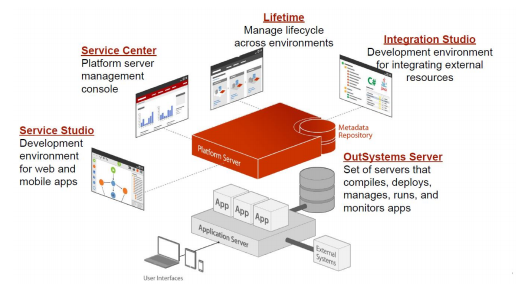
\includegraphics[width=\linewidth]{./figures/Architecture.png}
  \caption{OutSystems Architecture}\label{fig:architecture}
\end{figure}

\section*{Schedule} 

The project's management and schedule (Figure 2) will follow an agile [2] designated methodology, 
where the SCRUM framework [3] will be used since it is the most well-referenced and it enables to 
increase the productivity and quality of the development. 
Consequently, the project will be divided into cycles called Sprints, 
where the development of the project is focused on concluding an incremental solution that results 
from a previously established objective. Each incremental solution  is a fully functional, integrated, 
tested and documented application in which the final sprint will correspond to the delivery of the final product. 
In Figure 2 bellow, we can verify the schedule of all the sprints and phases included in the project.

\begin{figure}[H]
  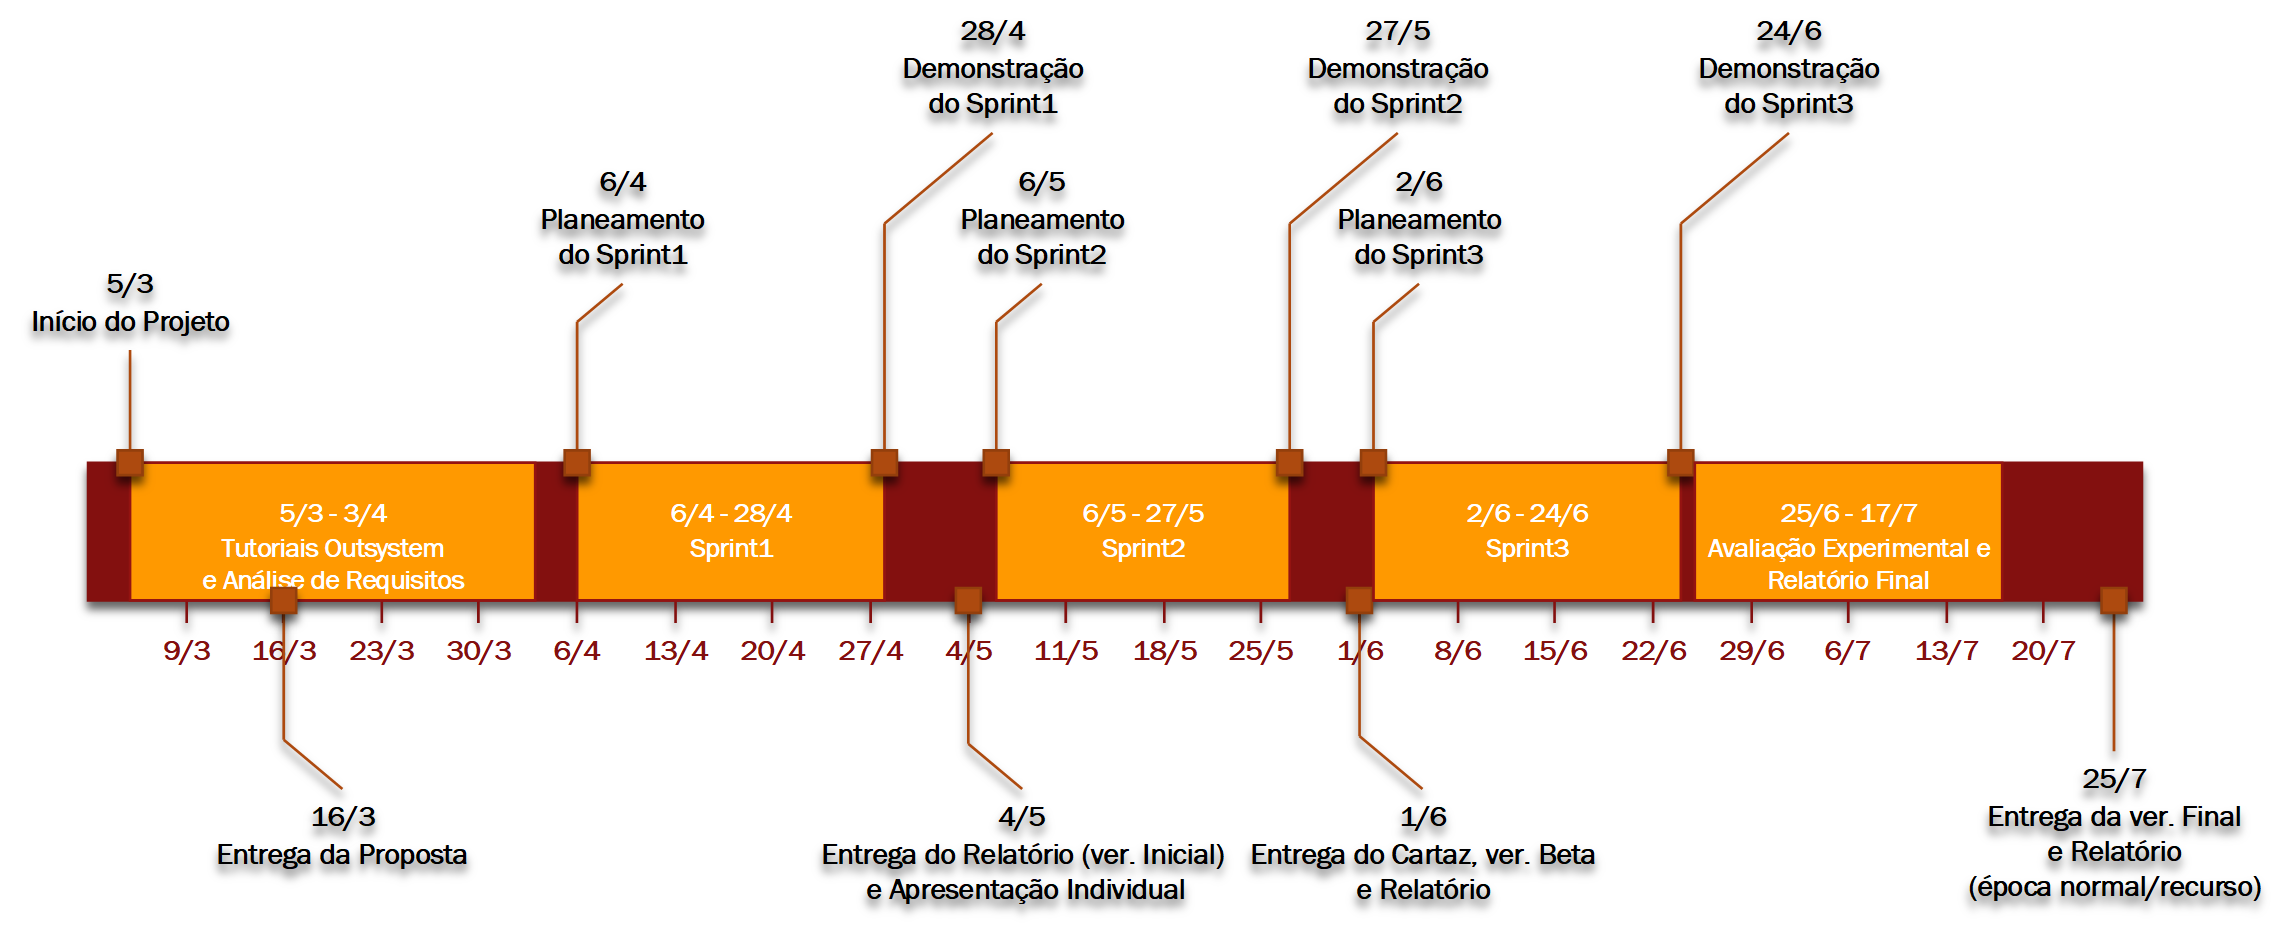
\includegraphics[width=\linewidth]{./figures/Timeline Projeto LEIC.png}
  \caption{Project Timeline}\label{fig:schedule}
\end{figure}

The initial phase of the project's development consists of making the OutSystems tutorials followed by a requirements analysis. 
The sprints that will be made while the development of the project will start with its planning and end with a demonstration 
and the elaboration of the project's report which will be made progressively throughout the sprints.

\section*{References}
\begin{enumerate}[label={[\arabic*]}]
  \item \url{https://www.outsystems.com/}
  \item \url{https://www.agilealliance.org/agile101/the-agile-manifesto}
  \item \url{https://www.scrum.org/resources/scrum-guide}
\end{enumerate}

\end{document}